\chapter{功能性需求}
\section{执行者分析}
各个执行者的关系如图~\ref{fig:roleRelation}所示。

在本项目中一共有四个角色,分别是难民,房主,编辑员和管理员。

房主继承难民,难民的所有功能房主都能拥有。难民即是游客,无需登陆注册就可以查看信息。游客想要成为房主需要注册登录并且完成实名认证才能够进行房源的发布,这是为了保障信息的真实有效性,来帮助更多的难民。
否则则默认是难民(游客)。

编辑员和管理员都属于管理层角色。编辑员拥有所有游客(难民)的基本功能,但是不能发布房源,因为编辑员默认没有登陆注册,只是有编辑新闻页面的权限,这里体现了权限管理。
管理者是系统中的权限最高的人物,所以同时拥有编辑员的所有权限,因此管理员继承自编辑员,但是拥有发布房源等救助信息、管理用户权限、管理角色权限的权限。

所以得到如图\ref{fig:roleRelation}所示的执行者关系图。
\begin{figure}[htbp]
    \centering
    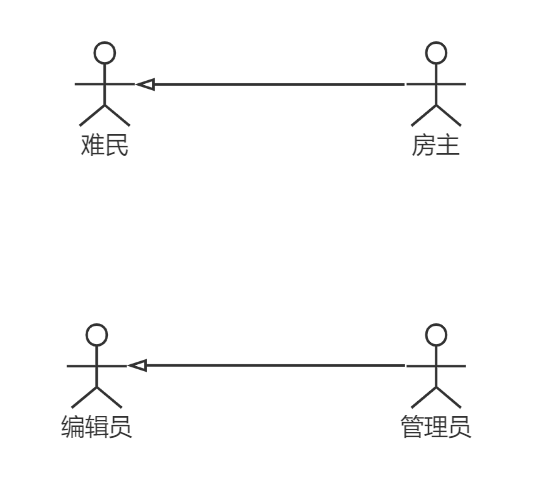
\includegraphics[width=0.8\textwidth]{ch5/roleRelation.png}
    \caption{执行者关系图}\label{fig:roleRelation}
    \vspace{\baselineskip} % 表示图与正文空一行
\end{figure}

\section{总用例图}
总用例图如图~\ref{fig:overallUseCase}~所示,其中包含了所有角色在系统中的功能,并且对于每一种角色这里只给出\textbf{第一层的用例图},详细的用例图会在接下来4个小节中详细介绍。

\begin{figure}[htbp]
    \centering
    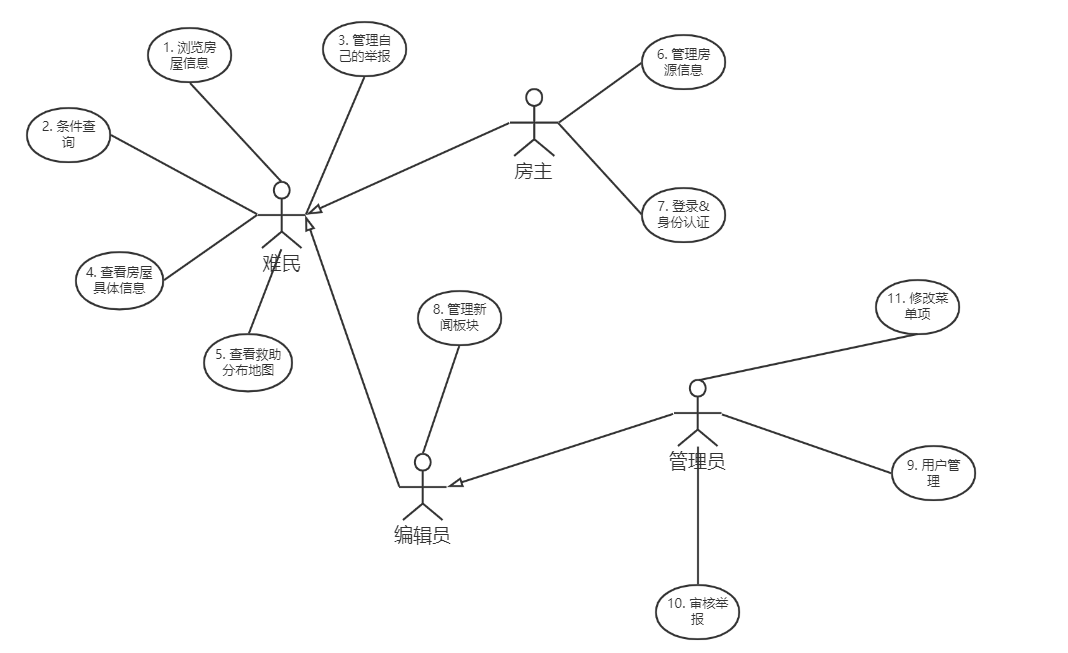
\includegraphics[width=\textwidth]{ch5/overallUseCase.png}
    \caption{总用例图}\label{fig:overallUseCase}
    \vspace{\baselineskip} % 表示图与正文空一行
\end{figure}

\section{难民用例图}

难民的用例图如图~\ref{fig:refugeeUseCase}~所示。

\begin{figure}[htbp]
    \centering
    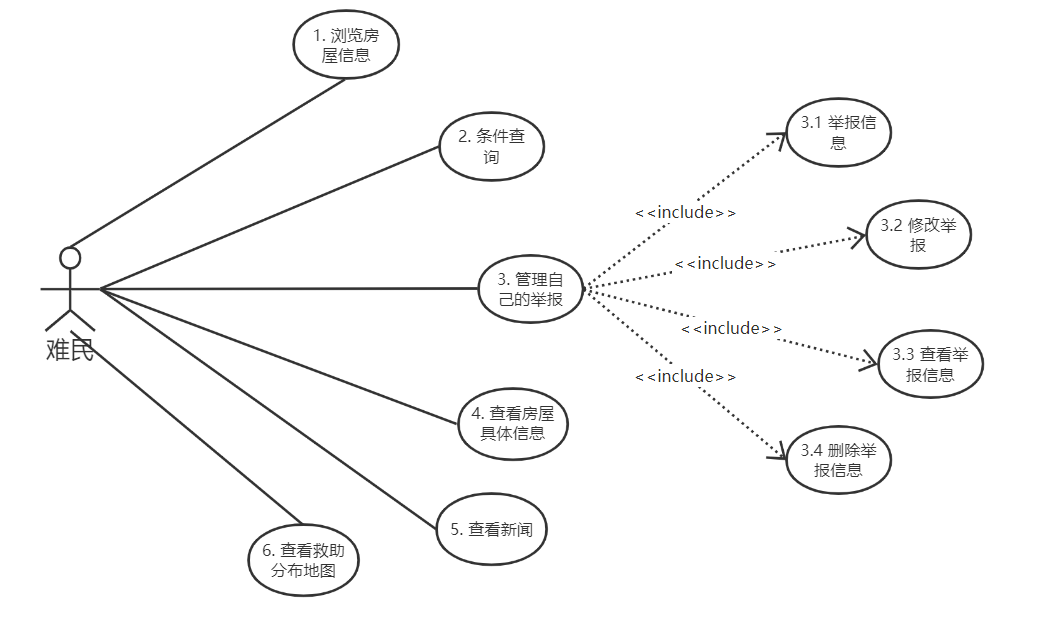
\includegraphics[width=0.8\textwidth]{ch5/refugeeUseCase.png}
    \caption{难民用例图}\label{fig:refugeeUseCase}
    \vspace{\baselineskip} % 表示图与正文空一行
\end{figure}

% 1 浏览房屋信息
\begin{table}[htbp]
    \centering
    \caption{浏览房屋信息}
    \vspace{0.5em}\wuhao
    \begin{tabular}{|l|l|l|l|}
        \hline
        \makebox[0.12\textwidth][l]{编号} & \makebox[0.25\textwidth][c]{UC-01 1}                      & \makebox[0.15\textwidth][l]{名称} & \makebox[0.3\textwidth][c]{浏览房屋信息} \\
        \hline
        执行者                            & \makebox[0.25\textwidth][c]{\makecell[c]{难民\quad房主                                                                                   \\编辑员\quad管理员}} & 优先级                            & \makebox[0.3\textwidth][c]{高 ~$\blacksquare$ ~中 ~$\square$~ 低 ~$\square$~} \\
        \hline
        描述                              & \multicolumn{3}{l|}{
        \begin{minipage}[t]{0.8\linewidth}
                目标:

                难民能够在浏览房主发布的房源信息概要和基本信息,选择匹配的房源。
也可以根据自己输入的地点来匹配地点附近的房源。

                具体要求:

                \begin{enumerate}[nosep]
                    \item 难民能看到具有简要信息的房源信息。
                    \item 房源信息需要按照发布时间逆序排列。
                    \item 房源信息以卡片的形式展现,需要展示如地址,入住要求等基本信息。
                    \item 需要有分页或者加载更多按钮来展现更多数据。
                          \vspace{0.5em}
                \end{enumerate}
            \end{minipage}     }                                                                                                                                             \\
        \hline
        前置条件                          & \multicolumn{3}{l|}{  房主发布房源信息并且录入数据库。  }                                                                                \\
        \hline
        基本流程                          & \multicolumn{3}{l|}{
        \begin{minipage}[t]{0.8\textwidth}
                \begin{enumerate}[nosep]
                    \item 进入房源信息页,查看信息。
                    \item 点击加载更多展示更多数据。
                          \vspace{0.5em}
                \end{enumerate}
            \end{minipage}     }                                                                                                                                             \\
        \hline
        结束状况                          & \multicolumn{3}{l|}{系统的数据不会发生变化。    }                                                                                        \\
        \hline
        可选流程                          & \multicolumn{3}{l|}{点击加载更多来展示更多数据。  }                                                                                      \\
        \hline
        异常流程                          & \multicolumn{3}{l|}{暂时没有可用的房源信息。    }                                                                                        \\
        \hline
        说明                              & \multicolumn{3}{l|}{无     }                                                                                                             \\
        \hline
    \end{tabular}
\end{table}

% 2 条件查询
\begin{table}[htbp]
    \centering
    \caption{条件查询}
    \vspace{0.5em}\wuhao
    \begin{tabular}{|l|l|l|l|}
        \hline
        \makebox[0.12\textwidth][l]{编号} & \makebox[0.25\textwidth][c]{UC-01 2}                      & \makebox[0.15\textwidth][l]{名称} & \makebox[0.3\textwidth][c]{条件查询} \\
        \hline
        执行者                            & \makebox[0.25\textwidth][c]{\makecell[c]{难民\quad房主                                                                               \\编辑员\quad管理员}}                       & 优先级                            & \makebox[0.3\textwidth][c]{高 ~$\blacksquare$ ~中 ~$\square$~ 低 ~$\square$~} \\
        \hline
        描述                              & \multicolumn{3}{l|}{
        \begin{minipage}[t]{0.8\linewidth}
                目标: 难民通过过滤器找到符合自己要求的房源等救助信息。
                \vspace{0.5em}
            \end{minipage}     }                                                                                                                                          \\
        \hline
        前置条件                          & \multicolumn{3}{l|}{  房主发布房源信息并且录入数据库。  }                                                                            \\
        \hline
        基本流程                          & \multicolumn{3}{l|}{
        \begin{minipage}[t]{0.8\textwidth}
                \begin{enumerate}[nosep]
                    \item 难民通过过滤器筛选条件。
                    \item 提交查询结果。
                    \item 显示查询成功并返回查询结果。
                          \vspace{0.5em}
                \end{enumerate}
            \end{minipage}     }                                                                                                                                         \\
        \hline
        结束状况                          & \multicolumn{3}{l|}{系统的数据不会发生变化。    }                                                                                    \\
        \hline
        可选流程                          & \multicolumn{3}{l|}{点击加载更多来展示更多数据。  }                                                                                  \\
        \hline
        异常流程                          & \multicolumn{3}{l|}{暂时没有相关的房源信息。 }                                                                                       \\
        \hline
        说明                              & \multicolumn{3}{l|}{无     }                                                                                                         \\
        \hline
    \end{tabular}
\end{table}

% 3 举报信息
\begin{table}[htbp]
    \centering
    \caption{举报信息}
    \vspace{0.5em}\wuhao
    \begin{tabular}{|l|l|l|l|}
        \hline
        \makebox[0.12\textwidth][l]{编号} & \makebox[0.25\textwidth][c]{UC-01 3-1}                                                           & \makebox[0.15\textwidth][l]{名称} & \makebox[0.3\textwidth][c]{举报信息}                                          \\
        \hline
        执行者                            & \makebox[0.25\textwidth][c]{难民\quad 房主}                                                      & 优先级                            & \makebox[0.3\textwidth][c]{高 ~$\blacksquare$ ~中 ~$\square$~ 低 ~$\square$~} \\
        \hline
        描述                              & \multicolumn{3}{l|}{\makecell[l]{难民/房主对于虚假不合规、房主违反提供住宿承诺的房源信息可以进行                                                                                                                     \\举报。}    }                                                                                                                     \\
        \hline
        前置条件                          & \multicolumn{3}{l|}{  房主发布房源信息并且录入数据库。难民能够看到房源信息。  }                                                                                                                                      \\
        \hline
        基本流程                          & \multicolumn{3}{l|}{
        \begin{minipage}[t]{0.8\textwidth}
                \begin{enumerate}[nosep]
                    \item 指示新建举报。
                    \item 显示举报申请表。
                    \item 填写申请单,选择请假类别。
                    \item 指示提交申请。
                    \item 显示成功提交申请的信息。
                          \vspace{0.5em}
                \end{enumerate}
            \end{minipage}     }                                                                                                                                                                                                                         \\
        \hline
        结束状况                          & \multicolumn{3}{l|}{系统保存举报的具体信息,并返回数据成功录入数据库的结果。    }                                                                                                                                    \\
        \hline
        可选流程                          & \multicolumn{3}{l|}{\begin{minipage}[t]{0.8\textwidth}
                \begin{enumerate}[nosep]
                    \item 指示取消举报。
                    \item 显示举报取消的信息。
                          \vspace{0.5em}
                \end{enumerate}
            \end{minipage}  }                                                                                                                                                                    \\
        \hline
        异常流程                          & \multicolumn{3}{l|}{   无}                                                                                                                                                                                           \\
        \hline
        说明                              & \multicolumn{3}{l|}{举报提交之后需要等待管理员审核并返回举报结果。    }                                                                                                                                              \\
        \hline
    \end{tabular}
\end{table}

% 4 修改举报信息
\begin{table}[htbp]
    \centering
    \caption{修改举报信息}
    \vspace{0.5em}\wuhao
    \begin{tabular}{|l|l|l|l|}
        \hline
        \makebox[0.12\textwidth][l]{编号} & \makebox[0.25\textwidth][c]{UC-01 3-2}                                                    & \makebox[0.15\textwidth][l]{名称} & \makebox[0.3\textwidth][c]{修改举报信息}                                      \\
        \hline
        执行者                            & \makebox[0.25\textwidth][c]{难民\quad 房主 \quad 编辑员}                                  & 优先级                            & \makebox[0.3\textwidth][c]{高 ~$\blacksquare$ ~中 ~$\square$~ 低 ~$\square$~} \\
        \hline
        描述                              & \multicolumn{3}{l|}{
        \begin{minipage}[t]{0.8\textwidth}
                目标:

                难民/房主/编辑员对于虚假不合规、房主违反提供住宿承诺的房源信息和不实的新闻可以进行举报。

                具体要求:

                \begin{enumerate}[nosep]
                    \item 举报申请提出以后,还没有任何审核之前,申请者可以修改请假申请。
                    \item 举报信息如果没有通过,申请者可以修改请假申请,重新提交。
                    \item 举报信息结果会以消息的形式发送到用户提交的联系方式中。
                          \vspace{0.5em}
                \end{enumerate}
            \end{minipage}     }                                                                                                                                                                                                                  \\
        \hline
        前置条件                          & \multicolumn{3}{l|}{  需存在已提交的举报信息。  }                                                                                                                                                             \\
        \hline
        基本流程                          & \multicolumn{3}{l|}{
        \begin{minipage}[t]{0.8\textwidth}
                \begin{enumerate}[nosep]
                    \item 查看自己的举报信息。
                    \item 点击某一具体举报信息的修改按钮。
                    \item 重新输入举报信息。
                    \item 重新提交。
                          \vspace{0.5em}
                \end{enumerate}
            \end{minipage}     }                                                                                                                                                                                                                  \\
        \hline
        结束状况                          & \multicolumn{3}{l|}{系统保存新提交的举报的具体信息,并返回数据成功录入数据库的结果。    }                                                                                                                     \\
        \hline
        可选流程                          & \multicolumn{3}{l|}{\begin{minipage}[t]{0.8\textwidth}
                \begin{enumerate}[nosep]
                    \item 指示取消举报。
                    \item 显示举报取消的信息。
                          \vspace{0.5em}
                \end{enumerate}
            \end{minipage}  }                                                                                                                                                             \\
        \hline
        异常流程                          & \multicolumn{3}{l|}{   无}                                                                                                                                                                                    \\
        \hline
        说明                              & \multicolumn{3}{l|}{举报提交之后需要等待管理员审核并返回举报结果。    }                                                                                                                                       \\
        \hline
    \end{tabular}
\end{table}

% 5 查看举报信息
\begin{table}[htbp]
    \centering
    \caption{查看举报信息}
    \vspace{0.5em}\wuhao
    \begin{tabular}{|l|l|l|l|}
        \hline
        \makebox[0.12\textwidth][l]{编号} & \makebox[0.25\textwidth][c]{UC-01 3-3}                   & \makebox[0.15\textwidth][l]{名称} & \makebox[0.3\textwidth][c]{查看举报信息}                                      \\
        \hline
        执行者                            & \makebox[0.25\textwidth][c]{难民\quad 房主 \quad 编辑员} & 优先级                            & \makebox[0.3\textwidth][c]{高 ~$\blacksquare$ ~中 ~$\square$~ 低 ~$\square$~} \\
        \hline
        描述                              & \multicolumn{3}{l|}{
        \begin{minipage}[t]{0.8\textwidth}
                目标:

                可以方便的查看自己的举报信息的审核情况,能查看自己的历史申请,在此基础上做下一步工作。

                具体要求:

                \begin{enumerate}[nosep]
                    \item 系统按照默认时间逆序显示当前用户的请假申请列表,用户可以通过该列表查看各举报的状态。
                    \item 举报申请可以按照时间的倒序或顺序排列,也可以按照举报的状态进行筛选。
                    \item 在查看申请的时候,角色可以查看或修改其中的一个具体的申请,或提出举报申请。
                    \item 用户在查看一个具体申请的时候才能删除该举报申请。
                          \vspace{0.5em}
                \end{enumerate}
            \end{minipage}     }                                                                                                                                                                                 \\
        \hline
        前置条件                          & \multicolumn{3}{l|}{用户有举报记录。 }                                                                                                                                       \\
        \hline

        结束状况                          & \multicolumn{3}{l|}{系统的数据不会发生变化。  }                                                                                                                              \\
        \hline
        异常流程                          & \multicolumn{3}{l|}{   无}                                                                                                                                                   \\
        \hline
        说明                              & \multicolumn{3}{l|}{无    }                                                                                                                                                  \\
        \hline
    \end{tabular}
\end{table}

% 6 删除举报信息
\begin{table}[htbp]
    \centering
    \caption{删除举报信息}
    \vspace{0.5em}\wuhao
    \begin{tabular}{|l|l|l|l|}
        \hline
        \makebox[0.12\textwidth][l]{编号} & \makebox[0.25\textwidth][c]{UC-01 3-4}                   & \makebox[0.15\textwidth][l]{名称} & \makebox[0.3\textwidth][c]{删除举报信息}                                      \\
        \hline
        执行者                            & \makebox[0.25\textwidth][c]{难民\quad 房主 \quad 编辑员} & 优先级                            & \makebox[0.3\textwidth][c]{高 ~$\blacksquare$ ~中 ~$\square$~ 低 ~$\square$~} \\
        \hline
        描述                              & \multicolumn{3}{l|}{删除自己的举报信息。   }                                                                                                                                 \\
        \hline
        前置条件                          & \multicolumn{3}{l|}{  需存在已提交的举报信息。  }                                                                                                                            \\
        \hline
        基本流程                          & \multicolumn{3}{l|}{
        \begin{minipage}[t]{0.8\textwidth}
                \begin{enumerate}[nosep]
                    \item 查看举报历史信息。
                    \item 点击查看具体举报信息。
                    \item 删除举报信息。
                          \vspace{0.5em}
                \end{enumerate}
            \end{minipage}     }                                                                                                                                                                                 \\
        \hline
        结束状况                          & \multicolumn{3}{l|}{系统删除指定的举报信息。    }                                                                                                                            \\
        \hline
        可选流程                          & \multicolumn{3}{l|}{
        \begin{minipage}[t]{0.8\textwidth}
                \begin{enumerate}[nosep]
                    \item 指示取消删除举报。
                    \item 显示举报删除取消的信息。
                          \vspace{0.5em}
                \end{enumerate}
            \end{minipage}  }                                                                                                                                                                                    \\
        \hline
        异常流程                          & \multicolumn{3}{l|}{ \begin{minipage}[t]{0.8\textwidth}
                \begin{enumerate}[nosep]
                    \item 指示删除举报。
                    \item 显示该举报正在受理或已受理完毕,无法删除。
                    \item 取消删除。
                          \vspace{0.5em}
                \end{enumerate}
            \end{minipage}}                                                                                                                             \\
        \hline
        说明                              & \multicolumn{3}{l|}{无    }                                                                                                                                                  \\
        \hline
    \end{tabular}
\end{table}

% 7 查看房源具体信息
\begin{table}[htbp]
    \centering
    \caption{查看房源具体信息}
    \vspace{0.5em}\wuhao
    \begin{tabular}{|l|l|l|l|}
        \hline
        \makebox[0.12\textwidth][l]{编号} & \makebox[0.25\textwidth][c]{UC-01 4}                                 & \makebox[0.15\textwidth][l]{名称} & \makebox[0.3\textwidth][c]{查看房源具体信息}                                  \\
        \hline
        执行者                            & \makebox[0.25\textwidth][c]{难民\quad 房主 \quad 编辑员}             & 优先级                            & \makebox[0.3\textwidth][c]{高 ~$\blacksquare$ ~中 ~$\square$~ 低 ~$\square$~} \\
        \hline
        描述                              & \multicolumn{3}{l|}{
        \begin{minipage}[t]{0.8\textwidth}
                用户可以查看房源的具体信息。
            \end{minipage}     }                                                                                                                                                                                             \\
        \hline
        前置条件                          & \multicolumn{3}{l|}{  房主发布了房源。  }                                                                                                                                                \\
        \hline
        基本流程                          & \multicolumn{3}{l|}{
        \begin{minipage}[t]{0.8\textwidth}
                \begin{enumerate}[nosep]
                    \item 查看房源信息列表。
                    \item 点击查看具体房源信息。
                          \vspace{0.5em}
                \end{enumerate}
            \end{minipage}     }                                                                                                                                                                                             \\
        \hline
        结束状况                          & \multicolumn{3}{l|}{系统的数据不会发生任何变化。    }                                                                                                                                    \\
        \hline
        可选流程                          & \multicolumn{3}{l|}{无 }                                                                                                                                                                 \\
        \hline
        异常流程                          & \multicolumn{3}{l|}{无}                                                                                                                                                                  \\
        \hline
        说明                              & \multicolumn{3}{l|}{房源信息列表要有基本的信息如地址,接纳条件等。 }                                                                                                                     \\
        \hline
    \end{tabular}
\end{table}

% 8 查看新闻
\begin{table}[htbp]
    \centering
    \caption{查看新闻}
    \vspace{0.5em}\wuhao
    \begin{tabular}{|l|l|l|l|}
        \hline
        \makebox[0.12\textwidth][l]{编号} & \makebox[0.25\textwidth][c]{UC-01 5}                         & \makebox[0.15\textwidth][l]{名称} & \makebox[0.3\textwidth][c]{查看新闻}                                          \\
        \hline
        执行者                            & \makebox[0.25\textwidth][c]{难民\quad 房主 \quad 编辑员}     & 优先级                            & \makebox[0.3\textwidth][c]{高 ~$\blacksquare$ ~中 ~$\square$~ 低 ~$\square$~} \\
        \hline
        描述                              & \multicolumn{3}{l|}{
        \begin{minipage}[t]{0.8\textwidth}
                用户可以查看新闻的具体信息。
            \end{minipage}     }                                                                                                                                                                                     \\
        \hline
        前置条件                          & \multicolumn{3}{l|}{  编辑员发布了新闻。  }                                                                                                                                      \\
        \hline
        基本流程                          & \multicolumn{3}{l|}{
        \begin{minipage}[t]{0.8\textwidth}
                \begin{enumerate}[nosep]
                    \item 查看新闻信息列表。
                    \item 点击查看具体新闻信息。
                          \vspace{0.5em}
                \end{enumerate}
            \end{minipage}     }                                                                                                                                                                                     \\
        \hline
        结束状况                          & \multicolumn{3}{l|}{系统的数据不会发生任何变化。    }                                                                                                                            \\
        \hline
        可选流程                          & \multicolumn{3}{l|}{无 }                                                                                                                                                         \\
        \hline
        异常流程                          & \multicolumn{3}{l|}{无}                                                                                                                                                          \\
        \hline
        说明                              & \multicolumn{3}{l|}{新闻列表要有基本的信息如标题,时间等。 }                                                                                                                     \\
        \hline
    \end{tabular}
\end{table}

% 9 查看救助地图
\begin{table}[htbp]
    \centering
    \caption{查看救助地图}
    \vspace{0.5em}\wuhao
    \begin{tabular}{|l|l|l|l|}
        \hline
        \makebox[0.12\textwidth][l]{编号} & \makebox[0.25\textwidth][c]{UC-01 6}                     & \makebox[0.15\textwidth][l]{名称} & \makebox[0.3\textwidth][c]{查看救助地图}                                      \\
        \hline
        执行者                            & \makebox[0.25\textwidth][c]{难民\quad 房主 \quad 编辑员} & 优先级                            & \makebox[0.3\textwidth][c]{高 ~$\square$ ~中 ~$\blacksquare$~ 低 ~$\square$~} \\
        \hline
        描述                              & \multicolumn{3}{l|}{
        \begin{minipage}[t]{0.8\textwidth}
                附近的救助信息,这些信息会以图标的形式在用户所在地的周围标注出来。
                \vspace{.5em}
            \end{minipage}     }                                                                                                                                                                                 \\
        \hline
        前置条件                          & \multicolumn{3}{l|}{  允许GPS定位。  }                                                                                                                                       \\
        \hline
        基本流程                          & \multicolumn{3}{l|}{无   }                                                                                                                                                   \\
        \hline
        结束状况                          & \multicolumn{3}{l|}{系统的数据不会发生任何变化。    }                                                                                                                        \\
        \hline
        可选流程                          & \multicolumn{3}{l|}{无 }                                                                                                                                                     \\
        \hline
        异常流程                          & \multicolumn{3}{l|}{无}                                                                                                                                                      \\
        \hline
        说明                              & \multicolumn{3}{l|}{
        \begin{minipage}[t]{0.8\textwidth}
                地图可以放大缩小,拖动,点击展示基本信息但是无法跳转,可以通过展示的基本信息进行条件查询。
                \vspace{.5em}
            \end{minipage} }                                                                                                                                                                                     \\
        \hline
    \end{tabular}
\end{table}

\section{房主用例图}

房主的用例图如图~\ref{fig:ownerUseCase}~所示。

\begin{figure}[htbp]
    \centering
    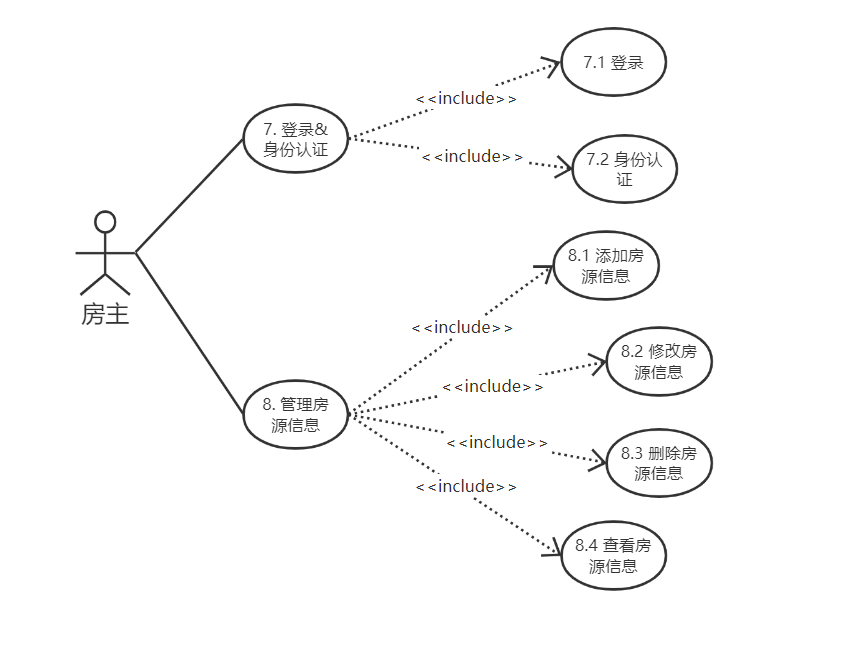
\includegraphics[width=.8\textwidth]{ch5/ownerUseCase.png}
    \caption{房主用例图}\label{fig:ownerUseCase}
    \vspace{\baselineskip} % 表示图与正文空一行
\end{figure}

% 10 登录
\begin{table}[htbp]
    \centering
    \caption{登录}
    \vspace{0.5em}\wuhao
    \begin{tabular}{|l|l|l|l|}
        \hline
        \makebox[0.12\textwidth][l]{编号} & \makebox[0.25\textwidth][c]{UC-02 7-1}                  & \makebox[0.15\textwidth][l]{名称} & \makebox[0.3\textwidth][c]{登录 \& 注册} \\
        \hline
        执行者                            & \makebox[0.25\textwidth][c]{\makecell[c]{难民\quad 房主                                                                                \\ 编辑员 \quad 管理员} }& 优先级                            & \makebox[0.3\textwidth][c]{高 ~$\blacksquare$ ~中 ~$\square$~ 低 ~$\square$~} \\
        \hline
        描述                              & \multicolumn{3}{l|}{部分功能需要用户登录才能操作。}                                                                                    \\
        \hline
        前置条件                          & \multicolumn{3}{l|}{  无  }                                                                                                            \\
        \hline
        基本流程                          & \multicolumn{3}{l|}{
            \begin{minipage}[t]{0.8\textwidth}
                \begin{enumerate}
                    \item 用户点击登录按钮。
                    \item 用户输入账号密码。
                    \item 登陆成功。
                \end{enumerate}
                \vspace{.5em}
            \end{minipage}
        }                                                                                                                                                                          \\
        \hline
        结束状况                          & \multicolumn{3}{l|}{数据库添加用户信息或改变状态。    }                                                                                \\
        \hline
        可选流程                          & \multicolumn{3}{l|}{无 }                                                                                                               \\
        \hline
        异常流程                          & \multicolumn{3}{l|}{
            \begin{minipage}[t]{0.8\textwidth}
                \begin{enumerate}
                    \item 账号密码没有输入,账号密码不匹配,用户名,密码不符合规范。
                    \item 弹出不规范提醒。
                    \item 重新登录或注册。
                \end{enumerate}
                \vspace{.5em}
            \end{minipage}
        }                                                                                                                                                                          \\
        \hline
        说明                              & \multicolumn{3}{l|}{
        \begin{minipage}[t]{0.8\textwidth}
                角色的有些功能需要登录,房主,编辑员和管理员必须登录。难民可以选择登录或者不登陆,如果难民不登陆,只能浏览房源信息,不能举报,查看举报信息等,此功能需要难民登录才能进行操作。
                \vspace{.5em}
            \end{minipage} }                                                                                                                                               \\
        \hline
    \end{tabular}
\end{table}

% 11 身份认证
\begin{table}[htbp]
    \centering
    \caption{身份认证}
    \vspace{0.5em}\wuhao
    \begin{tabular}{|l|l|l|l|}
        \hline
        \makebox[0.12\textwidth][l]{编号} & \makebox[0.25\textwidth][c]{UC-02 7-2}                        & \makebox[0.15\textwidth][l]{名称} & \makebox[0.3\textwidth][c]{身份认证} \\
        \hline
        执行者                            & \makebox[0.25\textwidth][c]{\makecell[c]{ 房主   \quad 编辑员                                                                            \\ 管理员} }& 优先级                            & \makebox[0.3\textwidth][c]{高 ~$\blacksquare$ ~中 ~$\square$~ 低 ~$\square$~} \\
        \hline
        描述                              & \multicolumn{3}{l|}{房主必须身份认证才能发布房源。}                                                                                      \\
        \hline
        前置条件                          & \multicolumn{3}{l|}{  无  }                                                                                                              \\
        \hline
        基本流程                          & \multicolumn{3}{l|}{
            \begin{minipage}[t]{0.8\textwidth}
                \begin{enumerate}
                    \item 点击be a host按钮
                    \item 依照提示上传ID证件
                    \item 认证完成
                \end{enumerate}
                \vspace{.5em}
            \end{minipage}
        }                                                                                                                                                                            \\
        \hline
        结束状况                          & \multicolumn{3}{l|}{数据库改变用户状态。    }                                                                                            \\
        \hline
        可选流程                          & \multicolumn{3}{l|}{无 }                                                                                                                 \\
        \hline
        异常流程                          & \multicolumn{3}{l|}{
            \begin{minipage}[t]{0.8\textwidth}
                \begin{enumerate}
                    \item 上传非法图片
                    \item 重新认证
                \end{enumerate}
                \vspace{.5em}
            \end{minipage}
        }                                                                                                                                                                            \\
        \hline
        说明                              & \multicolumn{3}{l|}{
        \begin{minipage}[t]{0.8\textwidth}
                本服务依赖stripe身份认证接口接口进行身份认证。如果无法调用国际身份认证接口,我们会调用阿里身份认证接口(支持国内)用于项目的演示,但是不意味着项目的初衷是使用阿里进行身份认证,我们将致力于使用合适国际身份认证接口。
                \vspace{.5em}
            \end{minipage} }                                                                                                                                                 \\
        \hline
    \end{tabular}
\end{table}

% 12 添加房源信息
\begin{table}[htbp]
    \centering
    \caption{添加房源信息}
    \vspace{0.5em}\wuhao
    \begin{tabular}{|l|l|l|l|}
        \hline
        \makebox[0.12\textwidth][l]{编号} & \makebox[0.25\textwidth][c]{UC-02 8-1}                  & \makebox[0.15\textwidth][l]{名称} & \makebox[0.3\textwidth][c]{添加房源信息}                                      \\
        \hline
        执行者                            & \makebox[0.25\textwidth][c]{房主 \quad 管理员}          & 优先级                            & \makebox[0.3\textwidth][c]{高 ~$\blacksquare$ ~中 ~$\square$~ 低 ~$\square$~} \\
        \hline
        描述                              & \multicolumn{3}{l|}{房主发布房源信息,为难民提供住所。}                                                                                                                     \\
        \hline
        前置条件                          & \multicolumn{3}{l|}{  房主完成身份认证。}                                                                                                                                   \\
        \hline
        基本流程                          & \multicolumn{3}{l|}{
            \begin{minipage}[t]{0.8\textwidth}
                \begin{enumerate}
                    \item 点击添加房源按钮。
                    \item 填写地址,接纳条件等信息
                    \item 发布并返回发布信息。
                \end{enumerate}
                \vspace{.5em}
            \end{minipage}
        }                                                                                                                                                                                                               \\
        \hline
        结束状况                          & \multicolumn{3}{l|}{数据库增加房源信息数据。    }                                                                                                                           \\
        \hline
        可选流程                          & \multicolumn{3}{l|}{点击取消按钮取消房源的发布。 }                                                                                                                          \\
        \hline
        异常流程                          & \multicolumn{3}{l|}{
            \begin{minipage}[t]{0.8\textwidth}
                \begin{enumerate}
                    \item 必填信息没有填写。
                    \item 重新填写并提交。
                \end{enumerate}
                \vspace{.5em}
            \end{minipage}
        }                                                                                                                                                                                                               \\
        \hline
        说明                              & \multicolumn{3}{l|}{
        \begin{minipage}[t]{0.8\textwidth}
                无
                \vspace{.5em}
            \end{minipage} }                                                                                                                                                                                    \\
        \hline
    \end{tabular}
\end{table}

% 13 修改房源信息
\begin{table}[htbp]
    \centering
    \caption{修改房源信息}
    \vspace{0.5em}\wuhao
    \begin{tabular}{|l|l|l|l|}
        \hline
        \makebox[0.12\textwidth][l]{编号} & \makebox[0.25\textwidth][c]{UC-02 8-2}             & \makebox[0.15\textwidth][l]{名称} & \makebox[0.3\textwidth][c]{修改房源信息}                                      \\
        \hline
        执行者                            & \makebox[0.25\textwidth][c]{房主 \quad 管理员}     & 优先级                            & \makebox[0.3\textwidth][c]{高 ~$\blacksquare$ ~中 ~$\square$~ 低 ~$\square$~} \\
        \hline
        描述                              & \multicolumn{3}{l|}{
        \begin{minipage}[t]{0.8\textwidth}
                \begin{enumerate}
                    \item 房主发布房源信息还没有和难民对接的时候,可以修改相关的信息。
                    \item 被通知举报成功之后需要重新填写信息并发布。
                \end{enumerate}
                \vspace{.5em}
            \end{minipage}}                                                                                                                                                                                \\
        \hline
        前置条件                          & \multicolumn{3}{l|}{  房主完成身份认证。}                                                                                                                              \\
        \hline
        基本流程                          & \multicolumn{3}{l|}{
            \begin{minipage}[t]{0.8\textwidth}
                \begin{enumerate}
                    \item   查看自己的房源列表。
                    \item 进入具体的房源编辑管理页面,修改并发布。
                \end{enumerate}
                \vspace{.5em}
            \end{minipage}
        }                                                                                                                                                                                                          \\
        \hline
        结束状况                          & \multicolumn{3}{l|}{数据库修改房源信息数据。    }                                                                                                                      \\
        \hline
        可选流程                          & \multicolumn{3}{l|}{点击取消按钮取消房源的修改。 }                                                                                                                     \\
        \hline
        异常流程                          & \multicolumn{3}{l|}{无}                                                                                                                                                \\
        \hline
        说明                              & \multicolumn{3}{l|}{无 }                                                                                                                                               \\
        \hline
    \end{tabular}
\end{table}

% 14 删除房源信息
\begin{table}[htbp]
    \centering
    \caption{删除房源信息}
    \vspace{0.5em}\wuhao
    \begin{tabular}{|l|l|l|l|}
        \hline
        \makebox[0.12\textwidth][l]{编号} & \makebox[0.25\textwidth][c]{UC-02 8-3}            & \makebox[0.15\textwidth][l]{名称} & \makebox[0.3\textwidth][c]{删除房源信息}                                      \\
        \hline
        执行者                            & \makebox[0.25\textwidth][c]{房主 \quad 管理员}    & 优先级                            & \makebox[0.3\textwidth][c]{高 ~$\blacksquare$ ~中 ~$\square$~ 低 ~$\square$~} \\
        \hline
        描述                              & \multicolumn{3}{l|}{
        \begin{minipage}[t]{0.8\textwidth}
                \begin{enumerate}
                    \item 查看发布的房源历史信息。
                    \item 点击查看具体房源信息。
                    \item 删除房源信息。
                \end{enumerate}
                \vspace{.5em}
            \end{minipage}}                                                                                                                                                                               \\
        \hline
        前置条件                          & \multicolumn{3}{l|}{  房主发布了房源信息。}                                                                                                                           \\
        \hline
        基本流程                          & \multicolumn{3}{l|}{
            \begin{minipage}[t]{0.8\textwidth}
                \begin{enumerate}
                    \item   查看自己的房源列表。
                    \item 进入具体的房源编辑管理页面,进行删除。
                \end{enumerate}
                \vspace{.5em}
            \end{minipage}
        }                                                                                                                                                                                                         \\
        \hline
        结束状况                          & \multicolumn{3}{l|}{数据库删除房源信息数据。    }                                                                                                                     \\
        \hline
        可选流程                          & \multicolumn{3}{l|}{无}                                                                                                                                               \\
        \hline
        异常流程                          & \multicolumn{3}{l|}{无}                                                                                                                                               \\
        \hline
        说明                              & \multicolumn{3}{l|}{
        \begin{minipage}[t]{0.8\textwidth}
                删除适用于找到了难民和房主主动删除两种情况,不过两种情况都由房主主动操作
                \vspace{0.5em}
            \end{minipage}   }                                                                                                                                                                            \\
        \hline
    \end{tabular}
\end{table}

% 15 查看房源信息
\begin{table}[htbp]
    \centering
    \caption{查看房源信息}
    \vspace{0.5em}\wuhao
    \begin{tabular}{|l|l|l|l|}
        \hline
        \makebox[0.12\textwidth][l]{编号} & \makebox[0.25\textwidth][c]{UC-02 8-4}               & \makebox[0.15\textwidth][l]{名称} & \makebox[0.3\textwidth][c]{查看房源信息}                                      \\
        \hline
        执行者                            & \makebox[0.25\textwidth][c]{房主 \quad 管理员}       & 优先级                            & \makebox[0.3\textwidth][c]{高 ~$\blacksquare$ ~中 ~$\square$~ 低 ~$\square$~} \\
        \hline
        描述                              & \multicolumn{3}{l|}{
        \begin{minipage}[t]{0.8\textwidth}
                目标:

                可以方便的查看自己的房源发布情况,在此基础上做下一步工作。
                \begin{enumerate}
                    \item 查看发布的房源历史信息。
                    \item 点击查看具体房源信息。
                \end{enumerate}
                \vspace{.5em}
            \end{minipage}}                                                                                                                                                                                  \\
        \hline
        前置条件                          & \multicolumn{3}{l|}{  房主发布了房源信息。}                                                                                                                              \\
        \hline
        基本流程                          & \multicolumn{3}{l|}{无}                                                                                                                                                  \\
        \hline
        结束状况                          & \multicolumn{3}{l|}{系统的数据不会发生任何变化。   }                                                                                                                     \\
        \hline
        可选流程                          & \multicolumn{3}{l|}{无}                                                                                                                                                  \\
        \hline
        异常流程                          & \multicolumn{3}{l|}{无}                                                                                                                                                  \\
        \hline
        说明                              & \multicolumn{3}{l|}{ 无}                                                                                                                                                 \\
        \hline
    \end{tabular}
\end{table}
\section{编辑员用例图}

编辑员的用例图如图~\ref{fig:editorUseCase}~所示。

\begin{figure}[htbp]
    \centering
    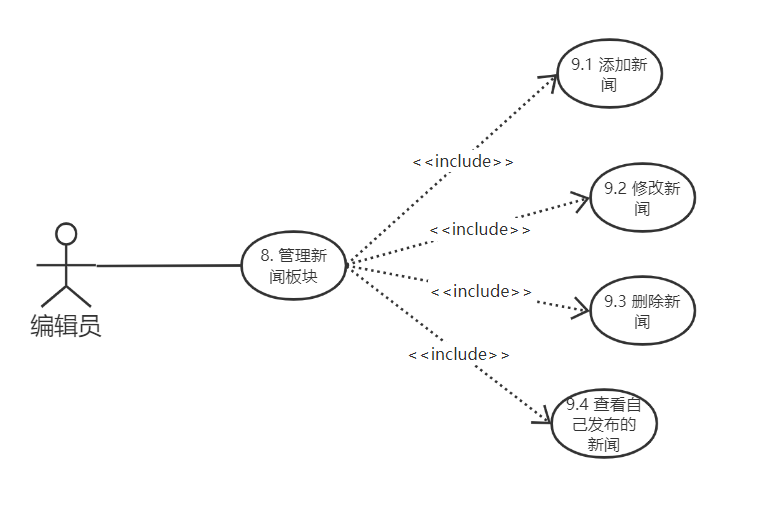
\includegraphics[width=.8\textwidth]{ch5/editorUseCase.png}
    \caption{编辑员用例图}\label{fig:editorUseCase}
    \vspace{\baselineskip} % 表示图与正文空一行
\end{figure}

% 16 添加新闻
\begin{table}[htbp]
    \centering
    \caption{添加新闻}
    \vspace{0.5em}\wuhao
    \begin{tabular}{|l|l|l|l|}
        \hline
        \makebox[0.12\textwidth][l]{编号} & \makebox[0.25\textwidth][c]{UC-03 9-1}                  & \makebox[0.15\textwidth][l]{名称} & \makebox[0.3\textwidth][c]{添加新闻}                                          \\
        \hline
        执行者                            & \makebox[0.25\textwidth][c]{编辑员}                     & 优先级                            & \makebox[0.3\textwidth][c]{高 ~$\square$ ~中 ~$\blacksquare$~ 低 ~$\square$~} \\
        \hline
        描述                              & \multicolumn{3}{l|}{编辑员即使发布战时新闻并做好分类。}                                                                                                                     \\
        \hline
        前置条件                          & \multicolumn{3}{l|}{无}                                                                                                                                                     \\
        \hline
        基本流程                          & \multicolumn{3}{l|}{
            \begin{minipage}[t]{0.8\textwidth}
                \begin{enumerate}
                    \item 点击添加新闻按钮。
                    \item 填写基本信息,并提交
                \end{enumerate}
                \vspace{.5em}
            \end{minipage}
        }                                                                                                                                                                                                               \\
        \hline
        结束状况                          & \multicolumn{3}{l|}{数据库增加新闻数据。    }                                                                                                                               \\
        \hline
        可选流程                          & \multicolumn{3}{l|}{点击取消按钮取消新闻的编辑发布。 }                                                                                                                      \\
        \hline
        异常流程                          & \multicolumn{3}{l|}{无}                                                                                                                                                     \\
        \hline
        说明                              & \multicolumn{3}{l|}{无}                                                                                                                                                     \\
        \hline
    \end{tabular}
\end{table}

% 17 修改新闻
\begin{table}[htbp]
    \centering
    \caption{修改新闻}
    \vspace{0.5em}\wuhao
    \begin{tabular}{|l|l|l|l|}
        \hline
        \makebox[0.12\textwidth][l]{编号} & \makebox[0.25\textwidth][c]{UC-03 9-2}               & \makebox[0.15\textwidth][l]{名称} & \makebox[0.3\textwidth][c]{修改新闻内容}                                      \\
        \hline
        执行者                            & \makebox[0.25\textwidth][c]{编辑员}                  & 优先级                            & \makebox[0.3\textwidth][c]{高 ~$\square$ ~中 ~$\blacksquare$~ 低 ~$\square$~} \\
        \hline
        描述                              & \multicolumn{3}{l|}{
        \begin{minipage}[t]{0.8\textwidth}
                新闻被举报并且审核通过之后或者编辑员想要自己修改,会下架新闻并通知编辑员修改新闻再次发布。
            \end{minipage}}                                                                                                                                                                                  \\
        \hline
        前置条件                          & \multicolumn{3}{l|}{无}                                                                                                                                                  \\
        \hline
        基本流程                          & \multicolumn{3}{l|}{
            \begin{minipage}[t]{0.8\textwidth}
                \begin{enumerate}
                    \item   查看自己发布的新闻列表。
                    \item 进入具体的新闻编辑管理页面,修改并发布。
                \end{enumerate}
                \vspace{.5em}
            \end{minipage}
        }                                                                                                                                                                                                            \\
        \hline
        结束状况                          & \multicolumn{3}{l|}{数据库修改新闻数据。    }                                                                                                                            \\
        \hline
        可选流程                          & \multicolumn{3}{l|}{点击取消按钮取消对新闻的修改。 }                                                                                                                     \\
        \hline
        异常流程                          & \multicolumn{3}{l|}{无}                                                                                                                                                  \\
        \hline
        说明                              & \multicolumn{3}{l|}{无}                                                                                                                                                  \\
        \hline
    \end{tabular}
\end{table}

% 18 删除新闻
\begin{table}[htbp]
    \centering
    \caption{删除新闻}
    \vspace{0.5em}\wuhao
    \begin{tabular}{|l|l|l|l|}
        \hline
        \makebox[0.12\textwidth][l]{编号} & \makebox[0.25\textwidth][c]{UC-03 9-3}                              & \makebox[0.15\textwidth][l]{名称} & \makebox[0.3\textwidth][c]{删除新闻信息}                                      \\
        \hline
        执行者                            & \makebox[0.25\textwidth][c]{编辑员}                                 & 优先级                            & \makebox[0.3\textwidth][c]{高 ~$\blacksquare$ ~中 ~$\square$~ 低 ~$\square$~} \\
        \hline
        描述                              & \multicolumn{3}{l|}{新闻被举报之后管理员会删除新闻并且通知管理员。}                                                                                                                     \\
        \hline
        前置条件                          & \multicolumn{3}{l|}{  编辑员发布了新闻信息。}                                                                                                                                           \\
        \hline
        基本流程                          & \multicolumn{3}{l|}{
            \begin{minipage}[t]{0.8\textwidth}
                \begin{enumerate}
                    \item   查看自己的新闻列表。
                    \item   进入具体的新闻编辑管理页面,进行删除。
                \end{enumerate}
                \vspace{.5em}
            \end{minipage}
        }                                                                                                                                                                                                                           \\
        \hline
        结束状况                          & \multicolumn{3}{l|}{数据库删除新闻信息数据。    }                                                                                                                                       \\
        \hline
        可选流程                          & \multicolumn{3}{l|}{取消删除。}                                                                                                                                                         \\
        \hline
        异常流程                          & \multicolumn{3}{l|}{无}                                                                                                                                                                 \\
        \hline
        说明                              & \multicolumn{3}{l|}{无}                                                                                                                                                                 \\
        \hline
    \end{tabular}
\end{table}

% 19 查看发布新闻
\begin{table}[htbp]
    \centering
    \caption{查看发布新闻}
    \vspace{0.5em}\wuhao
    \begin{tabular}{|l|l|l|l|}
        \hline
        \makebox[0.12\textwidth][l]{编号} & \makebox[0.25\textwidth][c]{UC-03 9-4}               & \makebox[0.15\textwidth][l]{名称} & \makebox[0.3\textwidth][c]{查看新闻信息}                                      \\
        \hline
        执行者                            & \makebox[0.25\textwidth][c]{编辑员}                  & 优先级                            & \makebox[0.3\textwidth][c]{高 ~$\blacksquare$ ~中 ~$\square$~ 低 ~$\square$~} \\
        \hline
        描述                              & \multicolumn{3}{l|}{
        \begin{minipage}[t]{0.8\textwidth}
                目标:


                可以方便的查看自己的房源发布情况,在此基础上做下一步工作。
                \begin{enumerate}
                    \item 查看发布的房源历史信息。
                    \item 点击查看具体房源信息。
                \end{enumerate}
                \vspace{.5em}
            \end{minipage}}                                                                                                                                                                                  \\
        \hline
        前置条件                          & \multicolumn{3}{l|}{房主发布了房源信息。}                                                                                                                                \\
        \hline
        基本流程                          & \multicolumn{3}{l|}{无}                                                                                                                                                  \\
        \hline
        结束状况                          & \multicolumn{3}{l|}{系统的数据不会发生任何变化。   }                                                                                                                     \\
        \hline
        可选流程                          & \multicolumn{3}{l|}{无}                                                                                                                                                  \\
        \hline
        异常流程                          & \multicolumn{3}{l|}{无}                                                                                                                                                  \\
        \hline
        说明                              & \multicolumn{3}{l|}{ 无}                                                                                                                                                 \\
        \hline
    \end{tabular}
\end{table}

\section{管理员用例图}

管理员的用例图如图~\ref{fig:adminUseCase}~所示。

\begin{figure}[htbp]
    \centering
    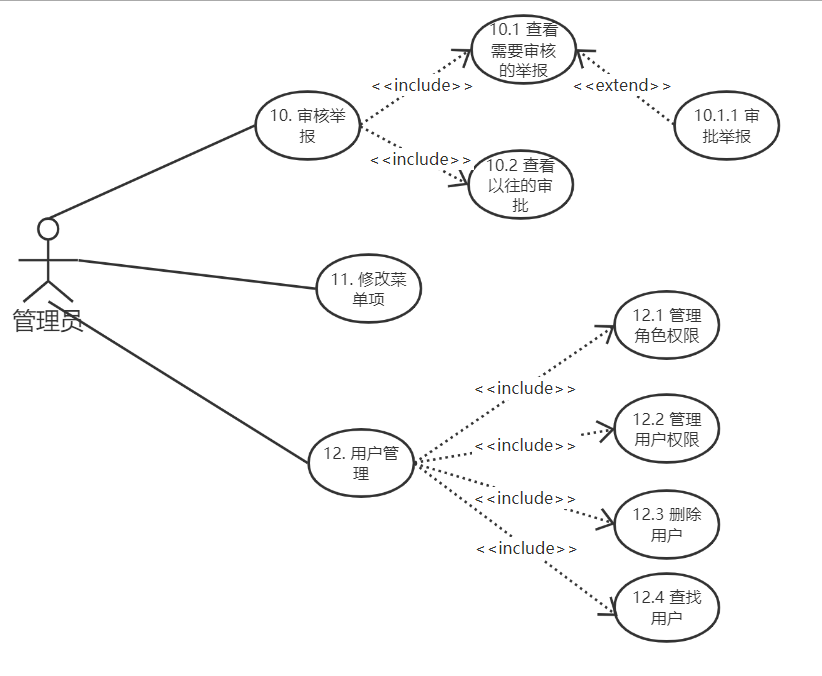
\includegraphics[width=.8\textwidth]{ch5/adminUseCase.png}
    \caption{管理员用例图}\label{fig:adminUseCase}
    \vspace{\baselineskip} % 表示图与正文空一行
\end{figure}

% 20 查看待审核举报
\begin{table}[htbp]
    \centering
    \caption{查看待审核举报}
    \vspace{0.5em}\wuhao
    \begin{tabular}{|l|l|l|l|}
        \hline
        \makebox[0.12\textwidth][l]{编号} & \makebox[0.25\textwidth][c]{UC-04 10-1 }             & \makebox[0.15\textwidth][l]{名称} & \makebox[0.3\textwidth][c]{查看待审核举报}                                    \\
        \hline
        执行者                            & \makebox[0.25\textwidth][c]{管理员}                  & 优先级                            & \makebox[0.3\textwidth][c]{高 ~$\blacksquare$ ~中 ~$\square$~ 低 ~$\square$~} \\
        \hline
        描述                              & \multicolumn{3}{l|}{
        \begin{minipage}[t]{0.8\textwidth}
                目标:

                部门经历需要方便的查看需要审核的申请,并在此基础上可以方便的审核。

                具体要求:
                \begin{enumerate}
                    \item 系统按照默认按照申请提出时间的顺序,列出状态为“待定”的举报申请列表。
                    \item 系统需要能够显示举报的基本信息。
                    \item 用户可以直接在举报列表界面审核通过,也可以在具体的举报界面审核。
                \end{enumerate}
                \vspace{.5em}
            \end{minipage}}                                                                                                                                                                                  \\
        \hline
        前置条件                          & \multicolumn{3}{l|}{有需要审核的举报。}                                                                                                                                  \\
        \hline
        结束状况                          & \multicolumn{3}{l|}{系统的数据不会发生任何变化。   }                                                                                                                     \\
        \hline
        可选流程                          & \multicolumn{3}{l|}{无}                                                                                                                                                  \\
        \hline
        说明                              & \multicolumn{3}{l|}{
            \begin{minipage}[t]{0.8\textwidth}
                \begin{enumerate}
                    \item 需要管理员审核的是状态为“待定”的申请。
                    \item 申请者提出举报申请之后,申请状态为“待定”。
                    \item 申请者修改被拒绝的举报之后,申请状态为“待定”。
                \end{enumerate}
                \vspace{.5em}
            \end{minipage}
        }                                                                                                                                                                                                            \\
        \hline
    \end{tabular}
\end{table}

% 21 审核举报
\begin{table}[htbp]
    \centering
    \caption{审核举报}
    \vspace{0.5em}\wuhao
    \begin{tabular}{|l|l|l|l|}
        \hline
        \makebox[0.12\textwidth][l]{编号} & \makebox[0.25\textwidth][c]{UC-04 10-1-1 }                                & \makebox[0.15\textwidth][l]{名称} & \makebox[0.3\textwidth][c]{审核举报}                                          \\
        \hline
        执行者                            & \makebox[0.25\textwidth][c]{管理员}                                       & 优先级                            & \makebox[0.3\textwidth][c]{高 ~$\blacksquare$ ~中 ~$\square$~ 低 ~$\square$~} \\
        \hline
        描述                              & \multicolumn{3}{l|}{
        \begin{minipage}[t]{0.8\textwidth}
                目标:

                用户能根据举报申请,审核该举报。

                具体要求:
                \begin{enumerate}
                    \item 用户可以直接在举报列表界面审核通过,也可以在具体的举报界面审核。
                    \item 审核的时候需要选择批准或拒绝,同时输入审核理由。
                    \item 审核时间不需要用户填入,由系统自动填入。
                \end{enumerate}
                \vspace{.5em}
            \end{minipage}}                                                                                                                                                                                                       \\
        \hline
        前置条件                          & \multicolumn{3}{l|}{有需要审核的举报。}                                                                                                                                                       \\
        \hline
        结束状况                          & \multicolumn{3}{l|}{系统根据用户的审核结果来更改数据库中对应消息的状态。}                                                                                                                     \\
        \hline
        可选流程                          & \multicolumn{3}{l|}{无}                                                                                                                                                                       \\
        \hline
        说明                              & \multicolumn{3}{l|}{无}                                                                                                                                                                       \\
        \hline
    \end{tabular}
\end{table}

% 22 查看以往的审核
\begin{table}[htbp]
    \centering
    \caption{查看以往的审核}
    \vspace{0.5em}\wuhao
    \begin{tabular}{|l|l|l|l|}
        \hline
        \makebox[0.12\textwidth][l]{编号} & \makebox[0.25\textwidth][c]{UC-04 10-2 }          & \makebox[0.15\textwidth][l]{名称} & \makebox[0.3\textwidth][c]{查看审核}                                          \\
        \hline
        执行者                            & \makebox[0.25\textwidth][c]{管理员}               & 优先级                            & \makebox[0.3\textwidth][c]{高 ~$\square$ ~中 ~$\blacksquare$~ 低 ~$\square$~} \\
        \hline
        描述                              & \multicolumn{3}{l|}{
        \begin{minipage}[t]{0.8\textwidth}
                目标:

                用户能够方便的查看曾经审批过的举报。

                具体要求:
                \begin{enumerate}
                    \item 系统按照默认按照申请提出时间的顺序,列出状态为“待定”的举报申请列表。
                    \item 系统需要能够显示举报的基本信息和状态。
                \end{enumerate}
                \vspace{.5em}
            \end{minipage}}                                                                                                                                                                               \\
        \hline
        前置条件                          & \multicolumn{3}{l|}{无}                                                                                                                                               \\
        \hline
        结束状况                          & \multicolumn{3}{l|}{系统的数据不会发生任何变化。}                                                                                                                     \\
        \hline
        可选流程                          & \multicolumn{3}{l|}{无}                                                                                                                                               \\
        \hline
        说明                              & \multicolumn{3}{l|}{无}                                                                                                                                               \\
        \hline
    \end{tabular}
\end{table}

% 23 修改菜单项
\begin{table}[htbp]
    \centering
    \caption{修改菜单项}
    \vspace{0.5em}\wuhao
    \begin{tabular}{|l|l|l|l|}
        \hline
        \makebox[0.12\textwidth][l]{编号} & \makebox[0.25\textwidth][c]{UC-04 11 }            & \makebox[0.15\textwidth][l]{名称} & \makebox[0.3\textwidth][c]{修改菜单项}                                        \\
        \hline
        执行者                            & \makebox[0.25\textwidth][c]{管理员}               & 优先级                            & \makebox[0.3\textwidth][c]{高 ~$\blacksquare$ ~中 ~$\square$~ 低 ~$\square$~} \\
        \hline
        描述                              & \multicolumn{3}{l|}{
        \begin{minipage}[t]{0.8\textwidth}
                目标:

                管理员能更改用户角色的菜单项

                具体要求:
                \begin{enumerate}
                    \item 管理员需要能够更改用户的下来菜单项。
                \end{enumerate}
                \vspace{.5em}
            \end{minipage}}                                                                                                                                                                               \\
        \hline
        前置条件                          & \multicolumn{3}{l|}{无}                                                                                                                                               \\
        \hline
        结束状况                          & \multicolumn{3}{l|}{系统的数据不会发生任何变化。}                                                                                                                     \\
        \hline
        说明                              & \multicolumn{3}{l|}{无}                                                                                                                                               \\
        \hline
    \end{tabular}
\end{table}

% 24 管理角色权限
\begin{table}[htbp]
    \centering
    \caption{管理角色权限}
    \vspace{0.5em}\wuhao
    \begin{tabular}{|l|l|l|l|}
        \hline
        \makebox[0.12\textwidth][l]{编号} & \makebox[0.25\textwidth][c]{UC-04 12.1 }                            & \makebox[0.15\textwidth][l]{名称} & \makebox[0.3\textwidth][c]{管理角色权限}                                      \\
        \hline
        执行者                            & \makebox[0.25\textwidth][c]{管理员}                                 & 优先级                            & \makebox[0.3\textwidth][c]{高 ~$\blacksquare$ ~中 ~$\square$~ 低 ~$\square$~} \\
        \hline
        描述                              & \multicolumn{3}{l|}{
        \begin{minipage}[t]{0.8\textwidth}
                目标:

                管理员能更改具体角色的权限
                \vspace{.5em}
            \end{minipage}}                                                                                                                                                                                                 \\
        \hline
        前置条件                          & \multicolumn{3}{l|}{无}                                                                                                                                                                 \\
        \hline
        基本流程                          & \multicolumn{3}{l|}{无}                                                                                                                                                                 \\
        \hline
        结束状况                          & \multicolumn{3}{l|}{用户角色权限发生变化。}                                                                                                                                             \\
        \hline
        异常流程                          & \multicolumn{3}{l|}{无}                                                                                                                                                                 \\
        \hline
        说明                              & \multicolumn{3}{l|}{管理员能够对于某一角色的用户的权限做集体更改。}                                                                                                                     \\
        \hline
    \end{tabular}
\end{table}

% 25 管理用户权限
\begin{table}[htbp]
    \centering
    \caption{管理用户权限}
    \vspace{0.5em}\wuhao
    \begin{tabular}{|l|l|l|l|}
        \hline
        \makebox[0.12\textwidth][l]{编号} & \makebox[0.25\textwidth][c]{UC-04 12-2 }                                      & \makebox[0.15\textwidth][l]{名称} & \makebox[0.3\textwidth][c]{管理用户权限}                                      \\
        \hline
        执行者                            & \makebox[0.25\textwidth][c]{管理员}                                           & 优先级                            & \makebox[0.3\textwidth][c]{高 ~$\blacksquare$ ~中 ~$\square$~ 低 ~$\square$~} \\
        \hline
        描述                              & \multicolumn{3}{l|}{
        \begin{minipage}[t]{0.8\textwidth}
                目标:

                管理员能更改具体某一用户的权限
                \vspace{.5em}
            \end{minipage}}                                                                                                                                                                                                           \\
        \hline
        前置条件                          & \multicolumn{3}{l|}{无}                                                                                                                                                                           \\
        \hline
        结束状况                          & \multicolumn{3}{l|}{用户权限发生变化。}                                                                                                                                                           \\
        \hline
        说明                              & \multicolumn{3}{l|}{管理员能够对于具体的用户的某些操作的权限进行剥夺和赋予。}                                                                                                                     \\
        \hline
    \end{tabular}
\end{table}

% 26 删除用户
\begin{table}[htbp]
    \centering
    \caption{删除用户}
    \vspace{0.5em}\wuhao
    \begin{tabular}{|l|l|l|l|}
        \hline
        \makebox[0.12\textwidth][l]{编号} & \makebox[0.25\textwidth][c]{UC-04 12-3 }                  & \makebox[0.15\textwidth][l]{名称} & \makebox[0.3\textwidth][c]{删除用户}                                          \\
        \hline
        执行者                            & \makebox[0.25\textwidth][c]{管理员}                       & 优先级                            & \makebox[0.3\textwidth][c]{高 ~$\blacksquare$ ~中 ~$\square$~ 低 ~$\square$~} \\
        \hline
        描述                              & \multicolumn{3}{l|}{管理员可以删除用户,禁止用户再次登录}                                                                                                                     \\
        \hline
        前置条件                          & \multicolumn{3}{l|}{无}                                                                                                                                                       \\
        \hline
        基本流程                          & \multicolumn{3}{l|}{无}                                                                                                                                                       \\
        \hline
        结束状况                          & \multicolumn{3}{l|}{修改用户在数据库中的状态。}                                                                                                                               \\
        \hline
        异常流程                          & \multicolumn{3}{l|}{无}                                                                                                                                                       \\
        \hline
        说明                              & \multicolumn{3}{l|}{
        \begin{minipage}[t]{0.8\textwidth}
                管理员对于用户的增删改查,增加的是编辑员账号信息;删除不合规的账号用户;对于用户的修改包括权限等在用例图UC-04 12-1 和12-2做了介绍.
                \vspace{.5em}
            \end{minipage}}                                                                                                                                                                                       \\
        \hline
    \end{tabular}
\end{table}

% 27 查找用户
\begin{table}[htbp]
    \centering
    \caption{删除用户}
    \vspace{0.5em}\wuhao
    \begin{tabular}{|l|l|l|l|}
        \hline
        \makebox[0.12\textwidth][l]{编号} & \makebox[0.25\textwidth][c]{UC-04 12-4 }                        & \makebox[0.15\textwidth][l]{名称} & \makebox[0.3\textwidth][c]{查找用户}                                          \\
        \hline
        执行者                            & \makebox[0.25\textwidth][c]{管理员}                             & 优先级                            & \makebox[0.3\textwidth][c]{高 ~$\square$ ~中 ~$\blacksquare$~ 低 ~$\square$~} \\
        \hline
        描述                              & \multicolumn{3}{l|}{管理员查找指定用户,在此基础上做继续操作。}                                                                                                                     \\
        \hline
        前置条件                          & \multicolumn{3}{l|}{无}                                                                                                                                                             \\
        \hline
        基本流程                          & \multicolumn{3}{l|}{无}                                                                                                                                                             \\
        \hline
        结束状况                          & \multicolumn{3}{l|}{修改用户在数据库中的状态。}                                                                                                                                     \\
        \hline
        异常流程                          & \multicolumn{3}{l|}{无}                                                                                                                                                             \\
        \hline
        说明                              & \multicolumn{3}{l|}{
        \begin{minipage}[t]{0.8\textwidth}
                查找用户,在在此基础上对用户的权限进行操作。
            \end{minipage}}                                                                                                                                                                                             \\
        \hline
    \end{tabular}
\end{table}

\newpage
\section{其他功能性需求}

\begin{enumerate}
    \item 房主发布房源需要身份认证,对于合适的国际身份认证平台还在寻找,在本项目中我们会暂时使用来登录阿里的身份认证来代替。
    \item 考虑是给世界的难民使用,所以需要由语言切换系统,本系统会采用谷歌翻译API来实现。
\end{enumerate}